\documentclass[9pt]{beamer}
\usefonttheme{professionalfonts}
\usetheme[subsectionpage=progressbar]{metropolis}
\setbeamertemplate{section in toc}[sections numbered]
\setbeamertemplate{subsection in toc}[subsections numbered]

\title{The Performance of \\ Physics Informed Neural Networks on \\ Metric Graphs}
\author{Tom-Christian Riemer}
\institute{TU Chemnitz}
\date{March 18th 2022}

%packages
\usepackage{amsmath}
\usepackage[british]{babel}
\usepackage[utf8]{inputenc}
\usepackage{enumerate}
\usepackage{graphicx}
\usepackage{mathtools}
\usepackage{color}
\usepackage{listings}
\usepackage{algpseudocode}
\usepackage{algorithm}
\usepackage{numapde-manifolds}
\usepackage{xcolor}
\usepackage{comment}
\usepackage{varwidth}
\usepackage{subcaption}
\usepackage{blkarray}
\usepackage{svg}
\usepackage{bold-extra}

\lstset{basicstyle=\ttfamily,	tabsize=2}

\newcommand\myeq{\stackrel{\mathclap{\mbox{$def$}}}{=}}

\newcommand{\Pb}[1]{\expandafter\hat#1}

\DeclareMathOperator*{\minimize}{minimize}

\begin{document}

\maketitle

\begin{frame}{Contents}
  \tableofcontents[hideallsubsections]
\end{frame}

\section{Introduction}

\begin{frame}{Yamal–Europe pipeline}
    \vspace{-1\baselineskip}\hfill{\tiny{[Wikipedia: Samuel Bailey (sam.bailus@gmail.com)]}}
    \begin{figure}[H]
        \begin{center}
            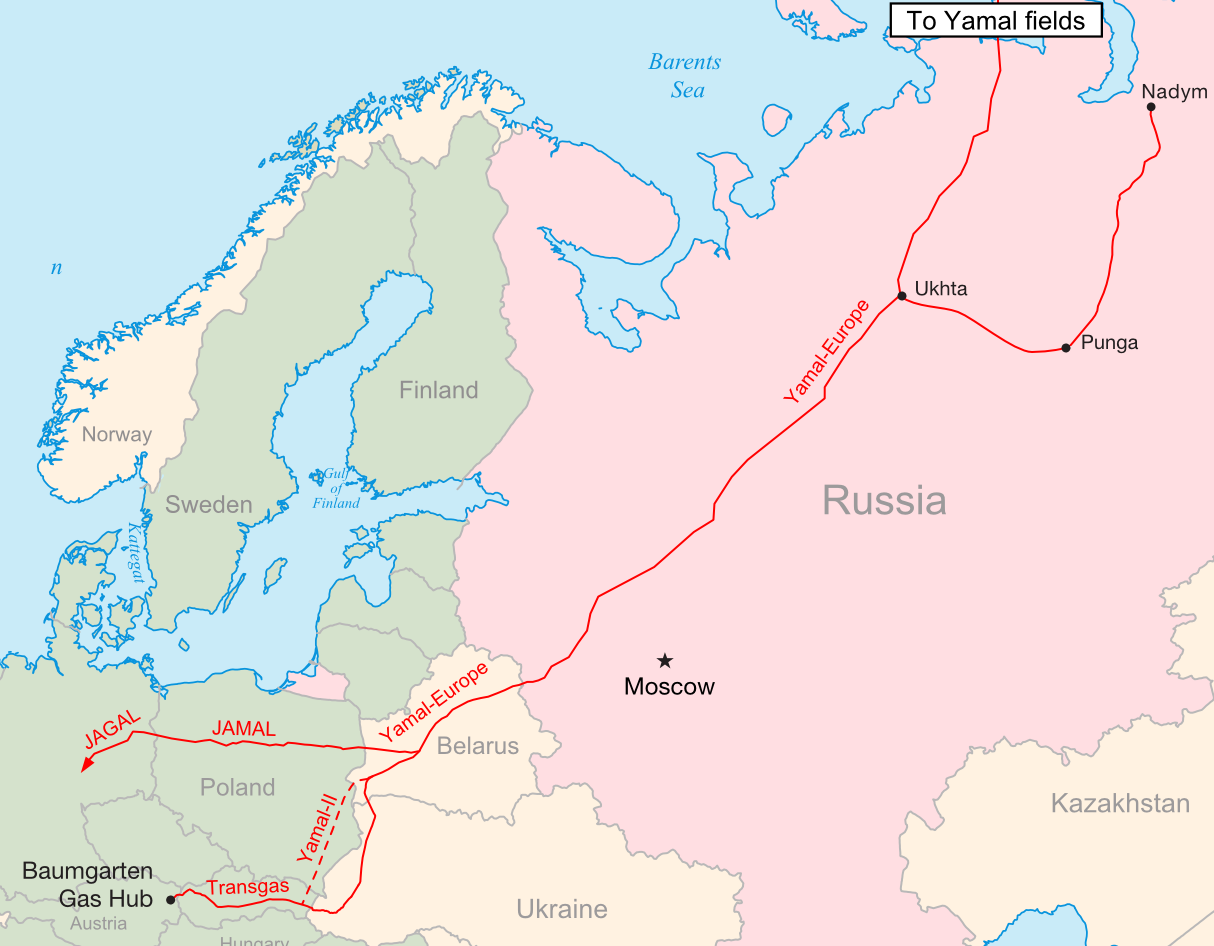
\includegraphics[scale=0.45]{img/Yamal-europe.png}
        \end{center}
    \end{figure}
\end{frame}

\section{Preliminaries}

\subsection{Metric Graphs}

\begin{frame}{Metric Graphs}
    \begin{minipage}{0.5\textwidth}
        \begin{itemize}
            \item $\Gamma = \left(\mathcal{V}, \mathcal{E} \right),$ \\ $\mathcal{V} = \left\{ v_i \right\}_{i = 1, \ldots, V}, \; V = \abs{\mathcal{V}} \in \mathbb{N},$ \\
            $\mathcal{E} = \left\{ e_i \right\}_{i = 1, \ldots, E}, \; E = \abs{\mathcal{E}} \in \mathbb{N}$.
            \item directed: $\forall e \in \mathcal{E} \colon \; e = \left( v^{\operatorname{o}}, v^{\operatorname{t}} \right)$ \\
            unique $v^{\operatorname{o}}, v^{\operatorname{t}} \in \mathcal{V}$.
            \item Reversal: $e_1, e_2 \in \mathcal{E} \colon e_1 = \overline{e_2}$ \\
            $\Leftrightarrow e_1 = \left( v_1, v_2 \right), e_2 = \left( v_2, v_1 \right)$.
        \end{itemize}
        \vspace{3mm}
        \textbf{Metric Graph}:
        \begin{itemize}
            \item $\forall e \in \mathcal{E} \colon \, \exists \ell_e > 0$.
            \item $\ell_{e_1} = \ell_{\overline{e_1}} = \ell_{e_2}$.
            \item $x_{e_1} \in [0, \ell_{e_1}]$.
            \item $\operatorname{dist}(v_i, v_j) = \sum^{N}_{k = 1} \ell_{e_k}$, \\ where $\left\{ e_k \right\}_{k = 1, \ldots, N}$ is path of minimal length.
        \end{itemize}
    \end{minipage} \hfill
    \begin{minipage}{0.45\textwidth}
        \begin{figure}[H]
            \resizebox{!}{!}
            {
                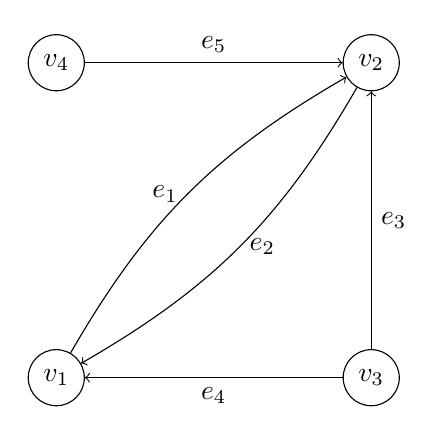
\begin{tikzpicture}
                    % vertices
                    \node[shape=circle,draw=black] (v4) at (0,4) {$v_4$};
                    \node[shape=circle,draw=black] (v2) at (4,4) {$v_2$};
                    \node[shape=circle,draw=black] (v1) at (0,0) {$v_1$};
                    \node[shape=circle,draw=black] (v3) at (4,0) {$v_3$};

                    % edges
                    \path [->](v3) edge node[below] {$e_4$} (v1);
                    \path [->](v2) edge [bend left = 15] node[right]{$e_2$} (v1);
                    \path [->](v1) edge [bend left = 15] node[left]{$e_1$} (v2);
                    \path [->](v3) edge node[right] {$e_3$} (v2);
                    \path [->](v4) edge node[above] {$e_5$} (v2);
                \end{tikzpicture}
            }
        \end{figure}
    \end{minipage}
\end{frame}



\begin{comment}
\begin{frame}{Metric Graphs}
    \vspace{-1\baselineskip}\hfill{\tiny{[Berkolaiko, Kuchment, 2013]}} \\
    \begin{minipage}{0.5\textwidth}
        \textbf{Metric Graph}:
        \begin{itemize}
            \item $\forall e \in \mathcal{E} \colon \, \exists \ell_e > 0$.
            \item $\ell_{e_1} = \ell_{\overline{e_1}} = \ell_{e_2} = \ell_{\tilde{e}}$.
            \item $x_{e_1} \in [0, \ell_{e_1}] \colon \, x_{e_1} = \ell_{e_2} - x_{e_2}$.
            \item $\operatorname{dist}(v_i, v_j) = \sum^{N}_{k = 1} \ell_{e_k}$, \\ where $\left\{ e_k \right\}_{k = 1, \ldots, N}$ is path of minimal length.
        \end{itemize}
    \end{minipage} \hfill
    \begin{minipage}{0.45\textwidth}
        \begin{figure}[H]
            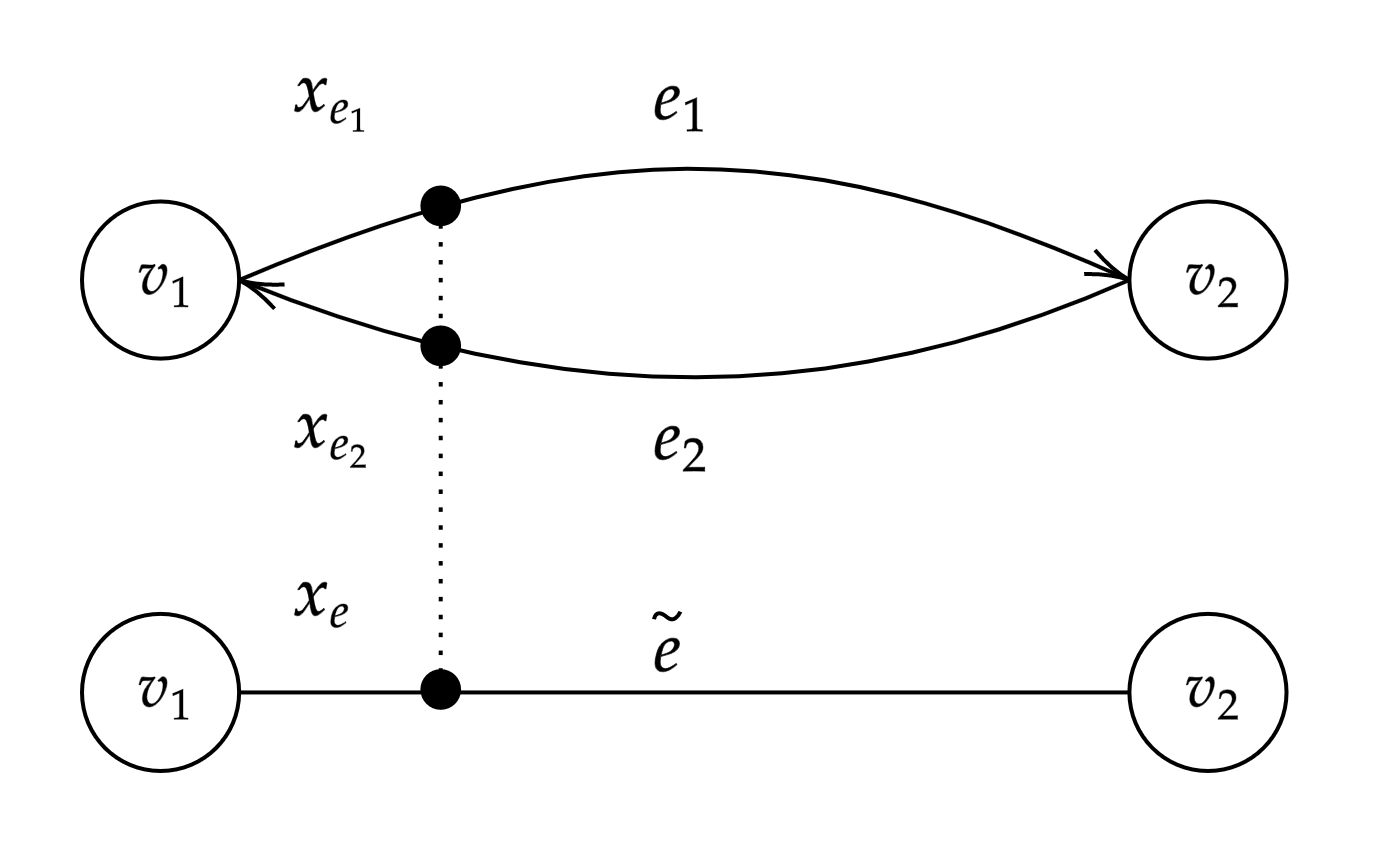
\includegraphics[scale=0.15]{img/diagram-20220315 (2).png}
        \end{figure}
    \end{minipage}
\end{frame}
\end{comment}



\begin{frame}{Function spaces}
    $L_2(e)$: \\
    \begin{equation*}
        \lVert f \rVert^{2}_{L_2(e)} \coloneqq \int_e \lvert f(x) \rvert^2 \, \textup{d} x < \infty.
    \end{equation*} \\
    $L_2(\Gamma) = \bigotimes_{e \in \mathcal{E}} L_2(e)$: \\
    \begin{equation*}
        \lVert f \rVert^{2}_{L_2(\Gamma)} \coloneqq \sum_{e \in \mathcal{E}} \lVert f \rVert^{2}_{L_2(e)} < \infty.
    \end{equation*} \\
    $H^1 (e)$: \\
    \begin{equation*}
        \lVert f \rVert^{2}_{H^1(e)} \coloneqq \int_e \lvert f(x) \rvert^2 + \lvert f^{\prime}(x) \rvert^2 \, dx < \infty.
    \end{equation*} \\
    $H^1 (\Gamma) =  \bigotimes_{e \in \mathcal{E}} H^1 (e) \cap C^{0}(\Gamma)$: \\
    \begin{equation*}
        \lVert f \rVert^{2}_{H^1 (\Gamma)} \coloneqq \sum_{e \in \mathcal{E}} \lVert f \rVert^{2}_{H^1 (e)} < \infty.
    \end{equation*}
\end{frame}



\subsection{Drift-Diffusion Equations}



\begin{frame}{Traffic flow}
    \begin{figure}[H]
        \begin{center}
            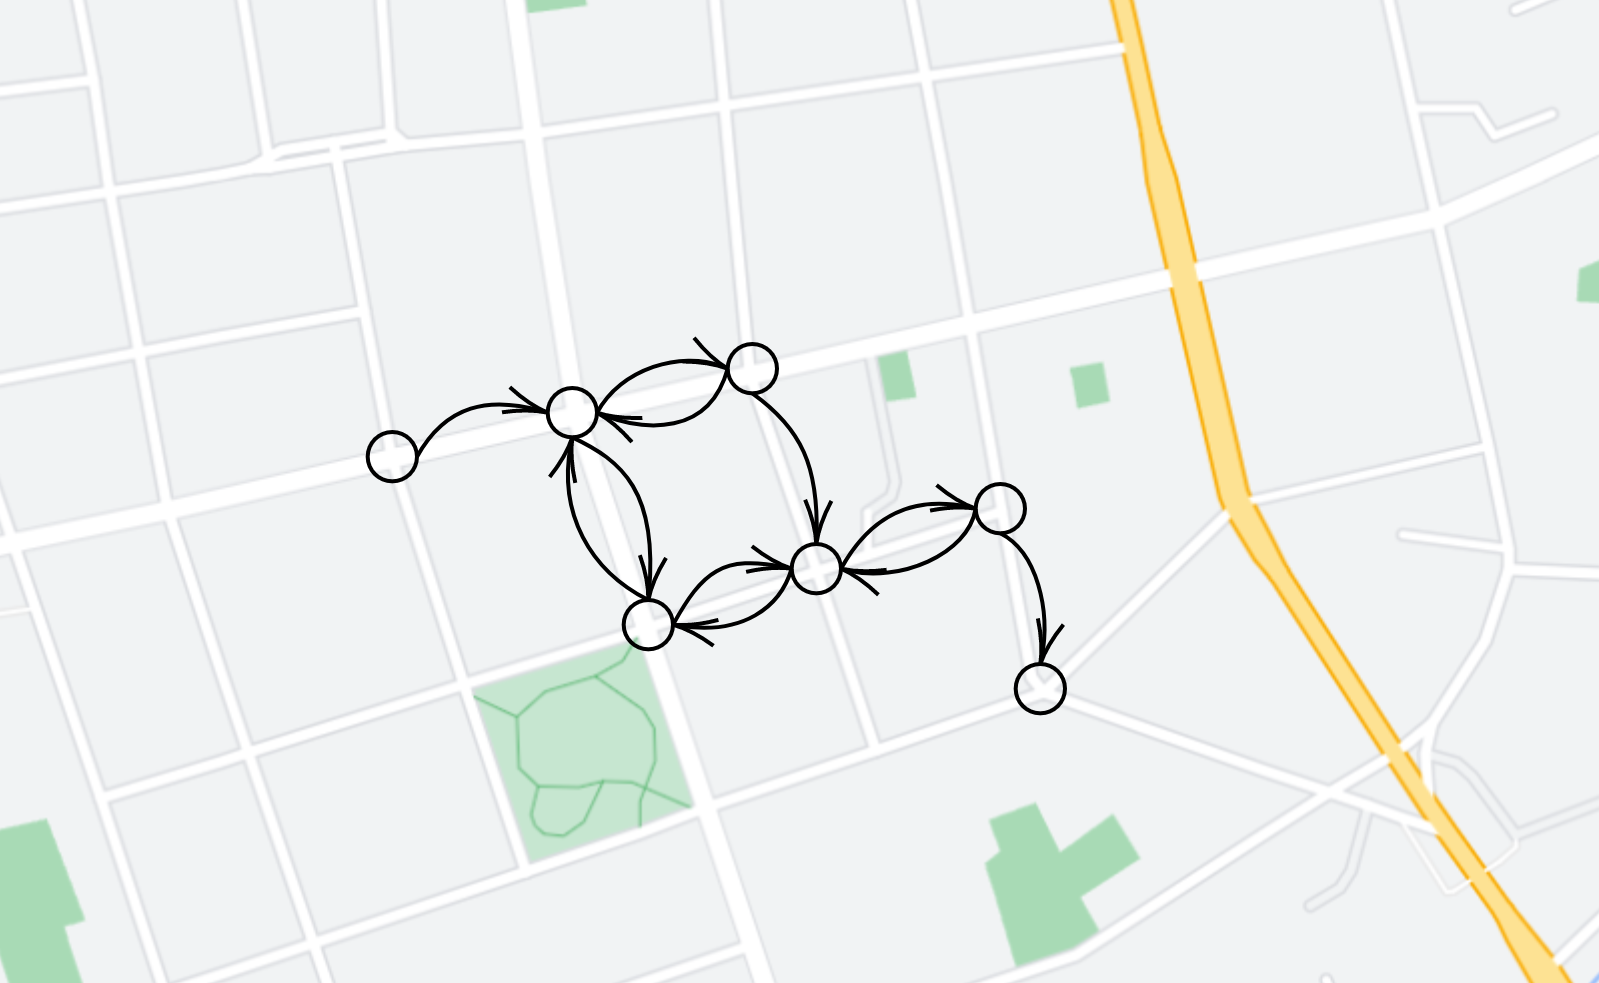
\includegraphics[scale=0.15]{img/diagram-20220316.png}
        \end{center}
    \end{figure}
    \begin{center}
        \small{A compact road network modelled by a compact metric graph}.
    \end{center}
    Continuity equation for each individual edge $e \in \mathcal{E}$:
    \begin{equation*}
        \partial_t \rho_e  \left( t,x \right)  = - \partial_x J_e \left( t,x \right).
    \end{equation*} \\
    \begin{itemize}
        \item Density of cars: $\rho_e \colon  \left( 0, T \right)  \times \left[ 0, \ell_e \right] \to \left[0, 1\right]$.
        \item Flux of cars: $J_e \colon  \left( 0,T \right)  \times \left[ 0, \ell_e \right] \to \mathbb{R}$.
    \end{itemize}
\end{frame}



\begin{frame}{Flux of cars}
    \begin{equation*} 
        J_e \left( t,x \right)  \coloneqq \underbrace{- \varepsilon \partial_x \rho_e  \left( t, x \right)}_{\text{diffusion}}  + \underbrace{f \left( \rho_e \left( t, x \right)  \right)  \partial_x V_e \left( t, x \right)}_{\text{drift}} 
    \end{equation*}
    \vspace{3mm}
    \begin{itemize}
        \item Diffusion coefficient $\varepsilon > 0$ (typically small).
        \item Potential $V_e \colon  \left( 0,T \right)  \times \left[ 0, \ell_e \right] \to \mathbb{R}_{+}$, that may vary from edge to edge.
        \item Mobility $f \colon \mathbb{R}_{+} \to \mathbb{R}_{+}, \; f \left( \rho_e \right)  =  \left( 1-\rho_e \right)  \rho_e \Rightarrow f \left( 0 \right)  = f \left( 1 \right)  = 0$. 
    \end{itemize}
\end{frame}



\begin{frame}{Drift-diffusion equations on a metric graph}
    Metric graph $\Gamma =  \left( \mathcal{V}, \mathcal{E} \right) $, where each edge $e \in \mathcal{E}$ is equipped with a length $\ell_e > 0$ and the following differential equation
    \begin{equation*} 
        \partial_t \rho_e  \left( t,x \right)  = \partial_x  \left( \varepsilon \partial_x \rho_e  \left( t,x \right)  - f \left( \rho_e  \left( t,x \right)   \right)  \partial_x V_e  \left( t,x \right)  \right), \; \forall \left( t,x \right) \in \left(0, T \right) \times \left[0, \ell_e \right].
    \end{equation*}
    $\Rightarrow$ For a well-posed problem we need initial and boundary conditions.

    \vspace{5mm}

    \textbf{Initial conditions}:
    \begin{equation*}
        \forall e \in \mathcal{E} \colon \; \rho_e \left( 0,x \right)  = \rho_{e, 0} \left( x \right) \in L^2 \left( e \right).
    \end{equation*}

    \vspace{3mm}

    The boundary conditions on a metric graph are \textbf{vertex conditions}!

    \vspace{3mm}

    \textbf{Normal vector}: $e = \left( v^{\operatorname{o}}_e, v^{\operatorname{t}}_e \right) \in \mathcal{E} \Rightarrow n_e \left( v^{\operatorname{o}}_e \right)  = -1, n_e \left( v^{\operatorname{t}}_e \right)  = 1$. \\

\end{frame}



\begin{frame}{Conditions on interior vertices}
    \textbf{Interior vertices}: \\
    $\forall v \in \mathcal{V}_\mathcal{K} \subset \mathcal{V} \colon \; \exists \ e_1 = \left( v^{\operatorname{o}}_{e_1}, v^{\operatorname{t}}_{e_1} \right), e_2 = \left( v^{\operatorname{o}}_{e_2}, v^{\operatorname{t}}_{e_2} \right) \in \mathcal{E}$ \\ s.t. $v^{\operatorname{t}}_{e_1} = v$ and $v^{\operatorname{o}}_{e_2} = v$. \\

    \vspace{5mm} 

    \textbf{Kirchhoff-Neumann conditions}:
    \begin{equation*}
        \forall v \in \mathcal{V}_\mathcal{K} \colon \; \sum_{e\in \mathcal{E}_v} J_e \left( t,v \right)  n_e  \left( v \right) =0,
    \end{equation*}
    where $\mathcal{E}_v$ the set of all edges incident to the vertex $v$. \\

    \vspace{5mm}

    \textbf{Continuity conditions}:
    \begin{equation*}
        \forall v \in \mathcal{V}_\mathcal{K} \colon \; \rho_e \left( v \right)  = \rho_{e'} \left( v \right), \; e,\,e' \in \mathcal{E}_v.
    \end{equation*}
\end{frame}



\begin{frame}{Conditions on exterior vertices}
    \textbf{Exterior vertices}: \\
    $\forall v \in \mathcal{V}_\mathcal{D} = \mathcal{V} \setminus \mathcal{V}_\mathcal{K} \colon$ either $v^{\operatorname{t}}_{e} = v$ or $v^{\operatorname{o}}_{e} = v$ holds $\forall e = \left(v^{\operatorname{o}}_{e}, v^{\operatorname{t}}_{e}\right) \in \mathcal{E}_v$ \\

    \vspace{5mm} 

    \textbf{Flux boundary conditions}:
    \begin{equation*}
        \forall v \in \mathcal{V}_\mathcal{D} \colon \; \sum_{e\in \mathcal{E}_v}J_e \left( t, v \right)  n_e  \left( v \right) =-\alpha_v \left( t \right)   \left( 1-\rho_e \left(t, v \right) \right)  + \beta_v \left( t \right)  \rho_e \left(t, v \right),
    \end{equation*}
    where 
    \begin{itemize}
        \item $\rho_e \left(t, v \right) = \rho_e \left(t, 0 \right)$ or $\rho_e \left(t, v \right) = \rho_e \left(t, \ell_e \right)$,
        \item $\alpha_v \colon  \left( 0,T \right)  \to \mathbb{R}_{+}$ influx rate,
        \item $\beta_v \colon  \left( 0,T \right)  \to \mathbb{R}_{+}$ outflux rate.
    \end{itemize}
    In typical situations: $\alpha_v \left( t \right)  \beta_v \left( t \right)  \equiv 0$ for all $v \in \mathcal{V}_\mathcal{D}$ and $t \in  \left( 0,T \right) $.
\end{frame}



\subsection{Neural Networks}



\begin{frame}{Artificial Neuron}
    \begin{figure}[H]
        \begin{center}
            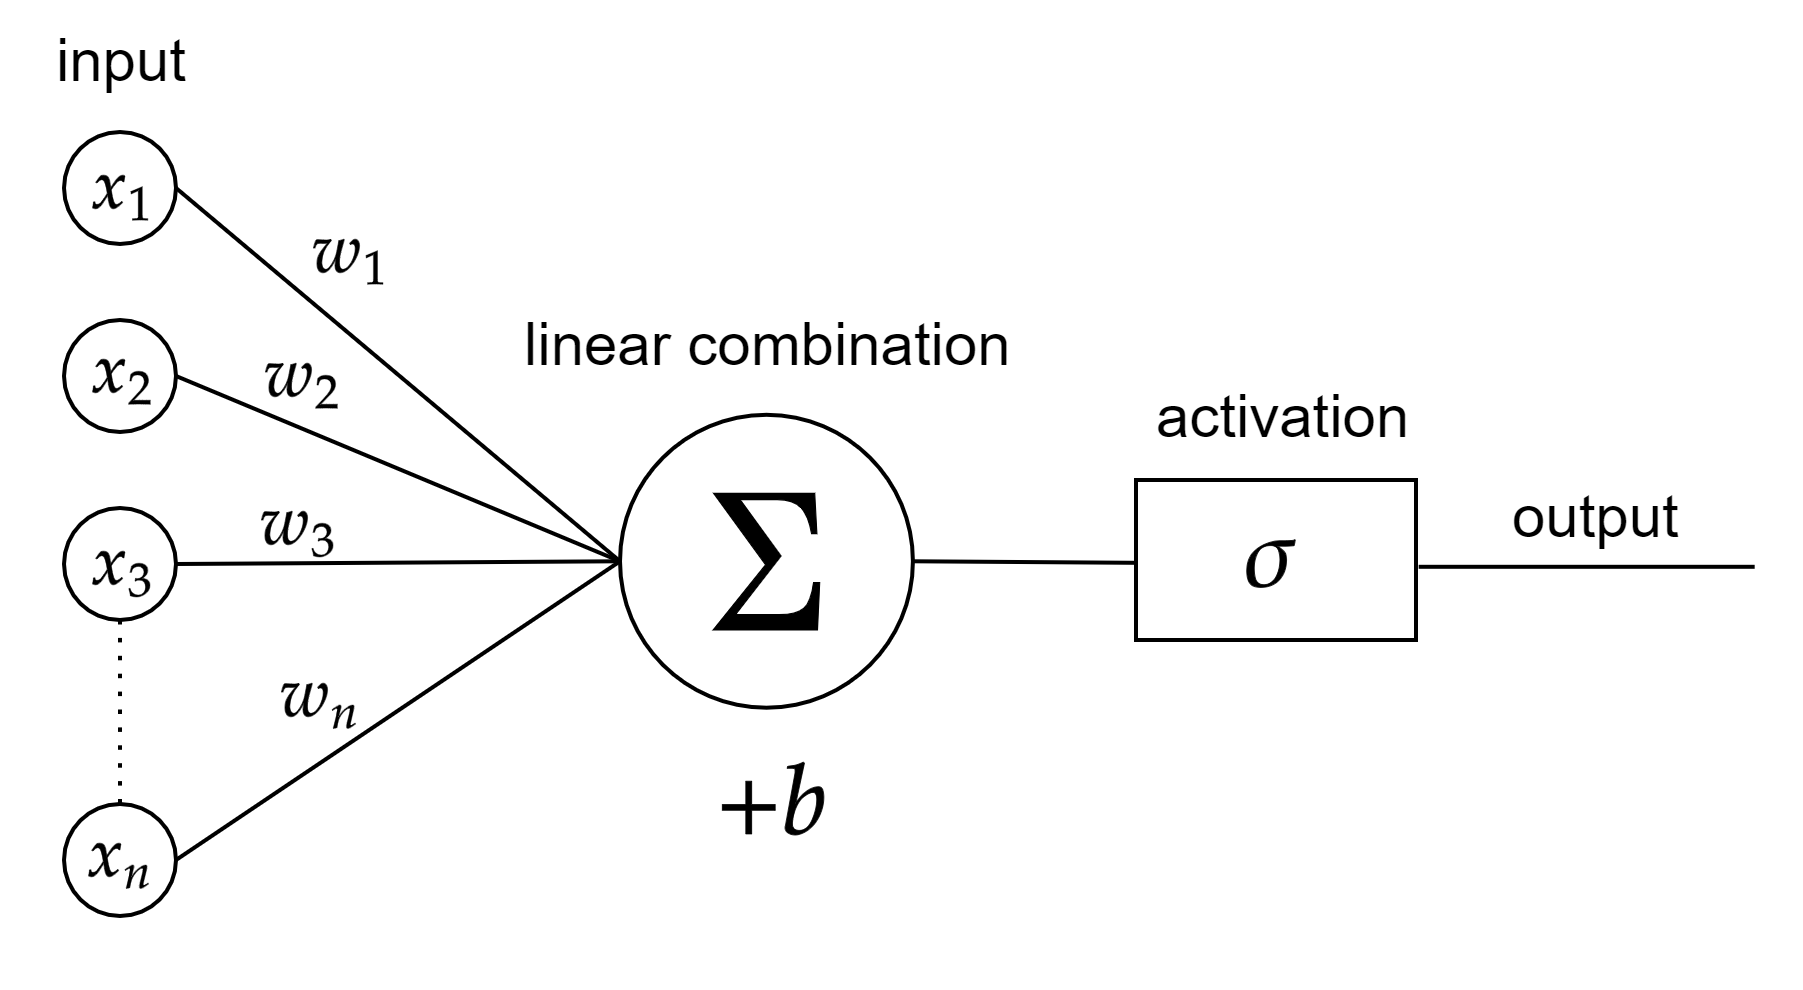
\includegraphics[scale=0.15]{img/diagram-20220205_1.png}
        \end{center}
    \end{figure}
    \begin{equation*}
        y = \sigma \left( \sum^{n}_{i=1} w_i x_i + b \right) = \sigma \left( w^{\mathrm{T}} x + b \right) = \sigma \left(a\right).
    \end{equation*}
    \begin{equation*}
        \begin{aligned}
            \sigma \left(a \right) &=\max \left\{ a, 0 \right\} & & \text{ rectified linear unit (ReLU) } \\
            \sigma \left(a\right) &=\frac{1}{1+\exp  \left(-a\right)} & & \text{ sigmoid }  \\
            \sigma \left(a\right) &=\tanh  \left(a\right)=\frac{\exp  \left(a\right)-\exp  \left(-a\right)}{\exp  \left(a\right)+\exp  \left(-a\right)} & & \text{ hyperbolic tangent }
        \end{aligned}
    \end{equation*}
\end{frame}

\begin{frame}{Feed-Forward Neural Network}
    \begin{figure}[H]
        \begin{center}
            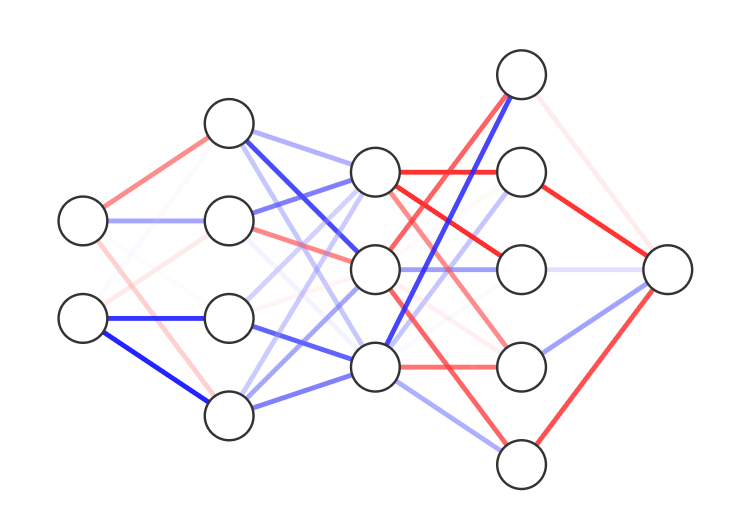
\includegraphics[scale=0.35]{img/Neural Network.png}
        \end{center}
    \end{figure}
    \begin{center}
        \small{“Neurons that fire together, wire together.” - Donald Hebb}
    \end{center}
    \begin{equation*}
        \begin{gathered}
            f_{\theta} \colon \mathbb{R}^{n_0} \to \mathbb{R}^{n_L}, \quad f_{\theta} \left( x^{0}\right) = x^{L} \\
            x^{l} = \sigma_l \left( W^l x^{l-1} + b^l \right) \quad \text{for} \quad l = 1, \ldots, L, 
        \end{gathered}
    \end{equation*}
    where 
    \begin{itemize}
        \item weights $W^l \in \mathbb{R}^{n_l \times n_{l-1}}$, biases $b^l \in \mathbb{R}^{n_l}$,
        \item trainable parameters $\theta = \left\{ \left\{ W^l \right\}_{l=1, \ldots, L}, \left\{ b^l \right\}_{l=1, \ldots, L} \right\}$,
        \item hyperparameter $L \in \mathbb{N}$ (depth), $n_l \in \mathbb{N}$ (width), $\sigma_l \colon \mathbb{R}^{n_l} \to \mathbb{R}^{n_l}$.
    \end{itemize}

\end{frame}



\begin{frame}{Machine Learning}
    \textbf{Supervised learning}: \\
    Training data $\left\{ \left(x_i, y_i \right) \right\}_{i = 1, \ldots, N}$ with $y_i = f(x_i)$. \\
    \begin{equation*}
        \minimize_{\theta} \; \frac{1}{N} \sum_{i=1}^{N} \lVert f_{\theta} \left(x_{i}\right) - y_{i} \rVert^{2}_2 =  MSE \left( \left\{ \left(x_i, y_i \right) \right\}_{i = 1, \ldots, N}, \theta \right).  
    \end{equation*}

    \vspace{3mm}

    \textbf{Stochastic gradient descent}: \\
    \begin{equation*}
        \label{Gradient Descent}
        \theta_{k+1} = \theta_k - \lambda \cdot \nabla_{\theta} MSE \left( \left(x_j, y_j \right), \theta_k \right),
    \end{equation*}
    where
    \begin{itemize}
        \item iterate $\theta_k$ in (large) search space,
        \item learning rate $\lambda > 0$,
        \item randomly chosen pair $\left(x_j, y_j \right)$ from $\left\{ \left(x_i, y_i \right) \right\}_{i = 1, \ldots, N}$,
        \item computation of $MSE \left( \left(x_j, y_j \right), \theta_k \right)$ with \textbf{back-propagation}. 
    \end{itemize}
\end{frame}



\subsection{Physics Informed Neural Networks}



\begin{frame}{Surrogate and Residual Network}
    \vspace{-1\baselineskip}\hfill{\tiny{[Raissi, Perdikaris, Karniadakis, 2017]}} \\
    Partial differential equation: \\
    \begin{equation*}
        \partial_t u\left(t,x\right) + \mathcal{H} \left[ u \right] \left(t, x\right) = 0, \quad x \in \Omega, \quad t \in \left[ 0, T \right].
    \end{equation*}

    \vspace{5mm}

    \textbf{Surrogate network}: \\
    \begin{equation*}
        u_\theta \left(t, x \right) \approx u\left(t,x\right) \; \text{ for all } \; \left(t, x \right) \in \left[ 0, T \right] \times \Omega.
    \end{equation*}
    
    \vspace{5mm}

    \textbf{Residual network}: \\
    \begin{equation*}
        r_{\theta} \left(t,x\right) = \partial_t u_{\theta} \left(t,x\right) + \mathcal{H} \left[ u_{\theta} \right] \left(t, x\right)
    \end{equation*}
    by using \textbf{automatic differentiation}.

\end{frame}



\begin{frame}{PINN Learning}

    \begin{figure}[H]
        \begin{center}
            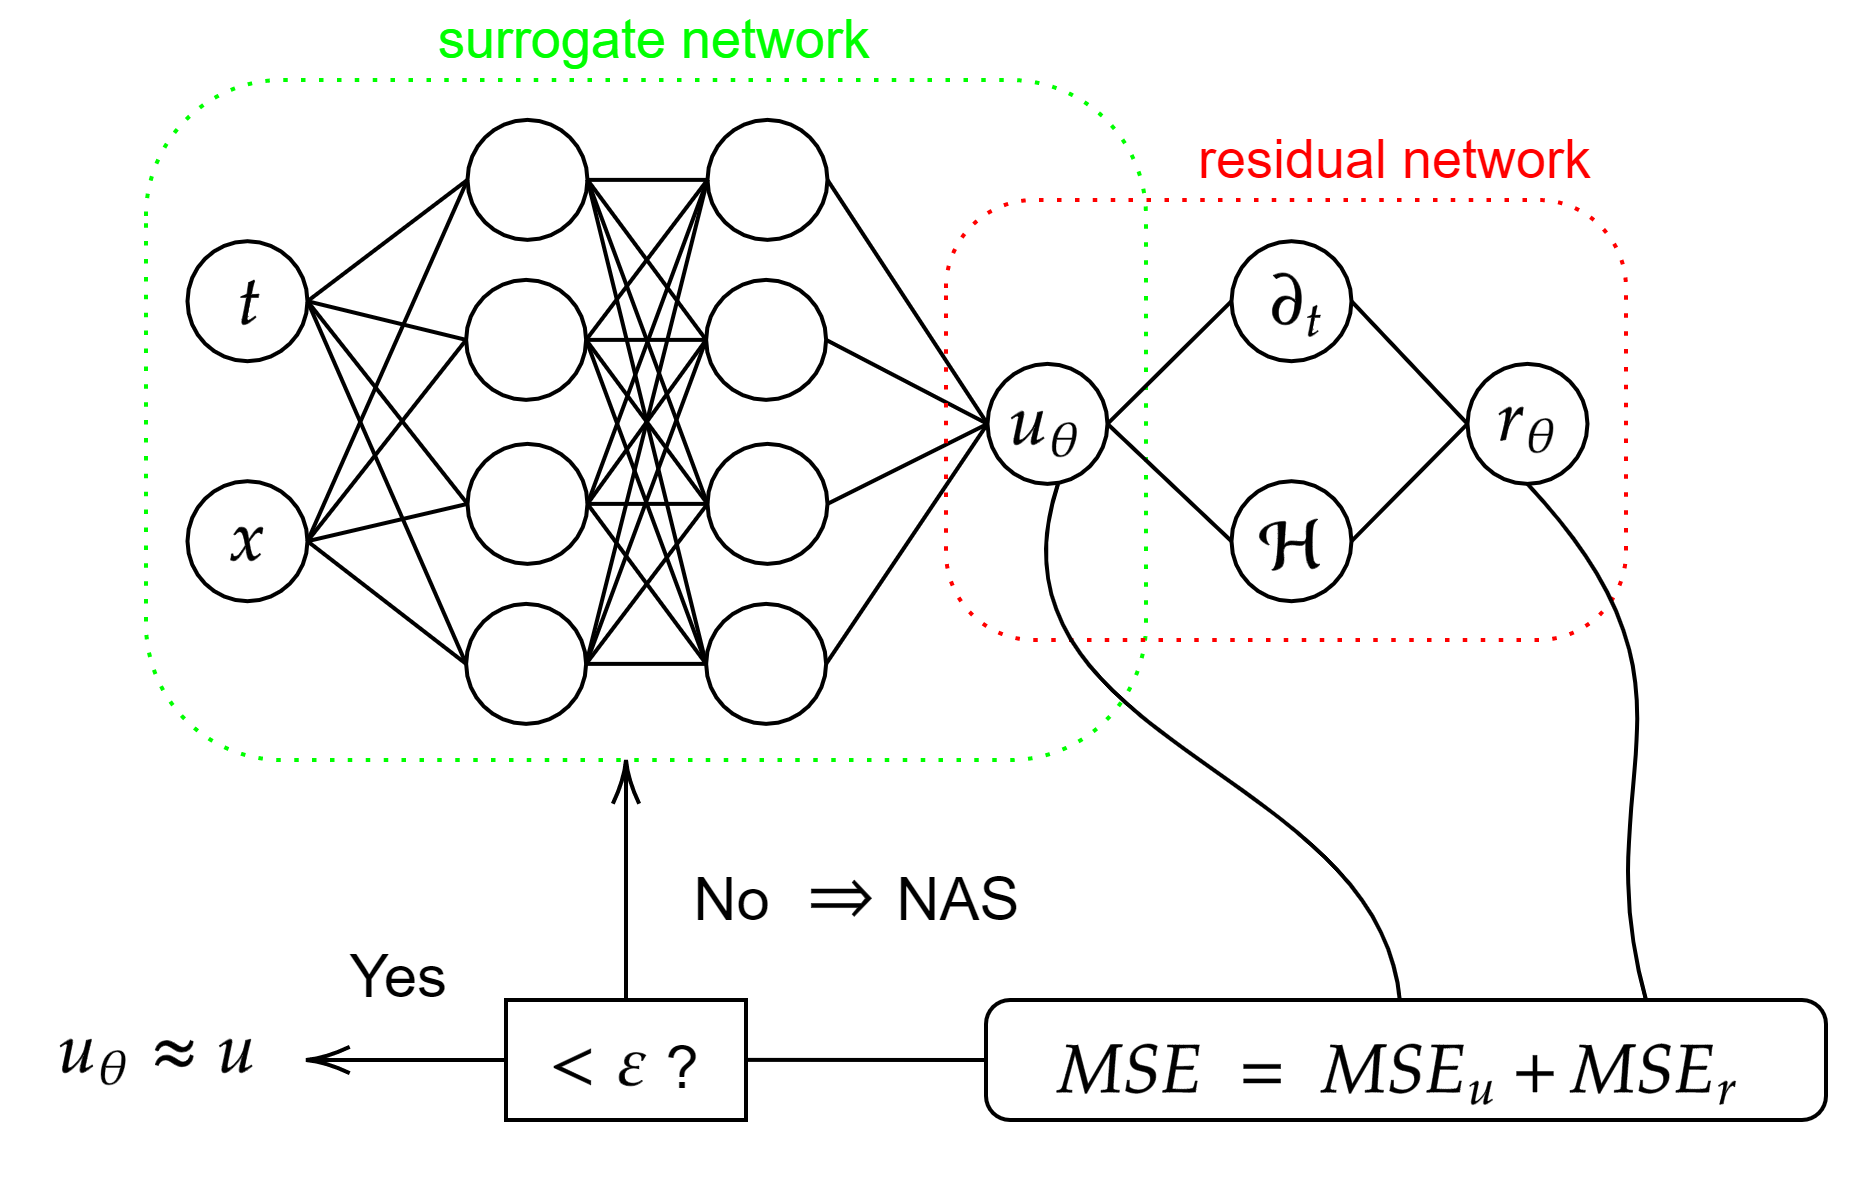
\includegraphics[scale=0.15]{img/PINN.png}
        \end{center}
    \end{figure}

    \textbf{Residual misfit term}: $MSE_r = \frac{1}{N_r} \sum^{N_r}_{i = 1} \lVert r_\theta \left(t^{r}_i, x^{r}_i\right) \rVert^{2}_{2}$ \\ 
    with collocation points $\left\{t^{r}_i, x^{r}_i \right\}_{i = 1, \ldots, N_r}$. 

    \textbf{Initial/Boundary misfit term}: $MSE_u = \frac{1}{N_u} \sum^{N_u}_{i = 1} \lVert u_\theta\left(t^{u}_i, x^{u}_i\right) - u_i \rVert^{2}_{2}$ \\
    with data $\left\{t^{u}_i, x^{u}_i, u_i \right\}_{i = 1, \ldots, N_u}$ (e.g. $u_i = u_0 \left(x^{u}_i\right)$). 
\end{frame}



\section{A PINN approach for solving \\ the set of Drift-Diffusion Equations \\ on a Metric Graph}



\begin{frame}{The “all at once” approach}
    \textbf{Surrogate network} $\rho_{\theta_e} \colon \mathbb{R}^2 \to \mathbb{R}$ approximates $\rho_e$ on each edge $e \in \mathcal{E}$. \\
    $\Rightarrow \; \theta_e$ are the trainable parameters that are involved in the approximation of $\rho_e$ on an individual edge $e \in \mathcal{E}$. \\
    \vspace{5mm}
    \textbf{Idea}: the set of drift-diffusion equations on all edges and all initial and vertex conditions are considered at once in the learning phase. \\
    \vspace{5mm}
    $\Rightarrow$ We construct one single cost function $\Phi_{\theta}$, which incorporates the deviations of all surrogate networks $\left\{\rho_{\theta_e} \right\}_{e \in \mathcal{E}}$ to$\ldots$
    \begin{itemize}
        \item $\ldots$the set of drift-diffusion equations on all edges $\mathcal{E}$,
        \item $\ldots$the initial conditions on all edges $e \in \mathcal{E}$,
        \item $\ldots$the vertex conditions on all vertices $v \in \mathcal{V}$.
    \end{itemize} 
\end{frame}



\begin{frame}{Deviation to the drift-diffusion equation}
    \textbf{Drift-diffusion equation} for each edge $e \in \mathcal{E}$
    \begin{equation*} 
        \partial_t \rho_e  \left( t,x \right)  = \partial_x  \left( \varepsilon \partial_x \rho_e  \left( t,x \right)  - f \left( \rho_e  \left( t,x \right)   \right)  \partial_x V_e  \left( t,x \right)  \right).
    \end{equation*}

    \vspace{3mm}

    \textbf{Residual network} for each edge $e \in \mathcal{E}$
    \begin{equation*}
        r_{\theta_e} \left( t,x \right)=\partial_t \rho_{\theta_e} \left( t,x \right) - \partial_x   \left(  \varepsilon \partial_x  \rho_{\theta_e} \left( t,x \right) - f \left( \rho_{\theta_e} \left( t,x \right) \right) \partial_x V \left( t,x \right) \right).
    \end{equation*}

    \vspace{3mm}

    \textbf{Residual misfit term} for each edge $e \in \mathcal{E}$
    \begin{equation*} 
        \phi_{e,r}  \left( X_e \right) \coloneqq \frac{1}{n_e} \sum_{i=1}^{n_e} r_{\theta_e}  \left( t_e^i, x_e^i  \right)^2,
    \end{equation*} 
    where $X_e = \left\{ \left( t_e^i, x_e^i \right) \right\}_{i=1}^{n_e} \subset \left( 0, T \right) \times \left[0, \ell_e\right]$ is a set of time-space collocation points. \\
\end{frame}



\begin{frame}{Deviation to the initial condition}
    \textbf{Initial conditions}:
    \begin{equation*}
        \forall e \in \mathcal{E} \colon \; \rho_e \left( 0,x \right)  = \rho_{e, 0} \left( x \right) \in L^2 \left( e \right).
    \end{equation*}

    \vspace{3mm}

    \textbf{Initial misfit term} for each edge $e \in \mathcal{E}$:
    \begin{equation*} 
        \phi_{e,0}  \left( X_{e,0} \right) \coloneqq \frac{1}{n_0} \sum_{i=1}^{n_0}  \left( \rho_{\theta_e}  \left( 0,x_{e,0}^i \right) - \rho_{e,0} \left( x_{e,0}^i \right) \right)^2, 
    \end{equation*} 
    where $X_{e,0} = \left\{ x_{e,0}^i \right\}_{i=1}^{n_0} \subset \left[0, \ell_e\right]$ is a set of collocation points along $t=0$.
\end{frame}



\begin{frame}{Deviation to the Kirchhoff-Neumann condition}
    \textbf{Kirchhoff-Neumann conditions}:
    \begin{equation*}
        \forall v \in \mathcal{V}_\mathcal{K} \colon \; \sum_{e\in \mathcal{E}_v} J_e \left( t,v \right)  n_e  \left( v \right) =0.
    \end{equation*}
    
    \vspace{3mm}

    \textbf{Kirchhoff-Neumann misfit term} for each interior vertex $v \in \mathcal{V}_{\mathcal{K}}$:
    \begin{equation*} 
        \phi_{v,K}  \left( X_{v,b} \right) \coloneqq \frac{1}{n_b} \sum_{i=1}^{n_b}  \left( \sum_{e \in \mathcal{E}_v}  J_{\theta_e}\left( t_{v,b}^i, v \right)  n_e  \left( v \right) \right)^2, 
    \end{equation*} 
    with 
    \begin{equation*} 
        J_{\theta_e}\left( t_{v,b}^i, v \right) = - \varepsilon \partial_x \rho_{\theta_e}  \left( t_{v,b}^i, v \right) + f \left( \rho_{\theta_e}  \left( t_{v,b}^i, v \right) \right) \partial_x V_e \left( t_{v,b}^i, v \right),
    \end{equation*}
    where $X_{v,b} = \left\{ t_{v,b}^i \right\}_{i=1}^{n_b} \subset \left( 0,T \right)$ is a set of time snapshots where the Kirchhoff-Neumann conditions are enforced.
\end{frame}



\begin{frame}{Deviation to the continuity condition}
    \textbf{Continuity conditions}:
    \begin{equation*}
        \forall v \in \mathcal{V}_\mathcal{K} \colon \; \rho_e \left( v \right)  = \rho_{e'} \left( v \right), \; e,\,e' \in \mathcal{E}_v.
    \end{equation*}

    \vspace{3mm}

    \textbf{Continuity misfit term} for each interior vertex $v \in \mathcal{V}_{\mathcal{K}}$:
    \begin{equation*} 
        \phi_{v,c}  \left( X_{v,b} \right) \coloneqq \frac{1}{n_b} \sum_{e \in \mathcal{E}_v} \sum_{i=1}^{n_b} \left(  \rho_{\theta_e}  \left( t_{v,b}^i, v \right) - \rho_{v}^i \right)^2,
    \end{equation*} 
    with $X_{v,b} = \left\{ t_{v,b}^i \right\}_{i=1}^{n_b}$ as introduced before and $\left\{ \rho_{v}^i \right\}_{i=1}^{n_b}$ additional trainable parameters for each $v \in \mathcal{V}_{\mathcal{K}}$, appended to $\theta$.
\end{frame}



\begin{frame}{Deviation to the flux boundary condition}
    \textbf{Flux boundary conditions}:
    \begin{equation*}
        \forall v \in \mathcal{V}_\mathcal{D} \colon \; \sum_{e\in \mathcal{E}_v}J_e \left( t, v \right)  n_e  \left( v \right) =-\alpha_v \left( t \right)   \left( 1-\rho_e \left(t, v \right) \right)  + \beta_v \left( t \right)  \rho_e \left(t, v \right).
    \end{equation*}

    \vspace{3mm}

    \textbf{Flux boundary misfit term} for each exterior vertex $v \in \mathcal{V}_{\mathcal{D}}$:
    \begin{equation*}
        \begin{aligned} 
            \phi_{v,D}  \left( X_{v,b} \right) \coloneqq & \frac{1}{n_b} \sum_{i=1}^{n_b} \bigg( \sum_{e \in \mathcal{E}_v} J_{\theta_e}\left( t_{v,b}^i, v \right) n_e  \left( v \right) + \\
            & \alpha_v \left( t_{v,b}^i \right)  \left( 1- \rho_{\theta_e}  \left( t_{v,b}^i, v \right) \right) - \beta_v \left( t_{v,b}^i \right) \rho_{\theta_e}  \left( t_{v,b}^i, v \right) \bigg)^2,
        \end{aligned}
    \end{equation*}
    with $X_{v,b} = \{t_{v,b}^i\}_{i=1}^{n_b}$ as introduced before.
\end{frame}



\begin{frame}{Final cost funktion}
    \begin{equation*}
        \begin{aligned} 
            \Phi_{\theta} \left( \operatorname{X} \right)  = & \quad \sum_{e \in \mathcal{E}}  \left(  \phi_{e,r}  \left( X_{e,r} \right) + \phi_{e,0}  \left( X_{e,0} \right)  \right) + \\
            & + \sum_{v \in \mathcal{V}_\mathcal{K}}  \left(  \phi_{v,K}  \left( X_{v,b} \right) + \phi_{v,c} \left( X_{v,b} \right)  \right) + \\
            & + \sum_{v \in \mathcal{V}_\mathcal{D}} \phi_{v,D} \left( X_{v,b} \right),
        \end{aligned}
    \end{equation*}
    where $\operatorname{X}$ is the union of the different collocation points $X_e$, $X_{v,b}$ and $X_{e,0}$. \\

    \vspace{5mm}

    $\Rightarrow$ The minimization of $\Phi_{\theta} \left( \operatorname{X} \right)$ with respect to the trainable parameters $\theta$ should ensure that the surrogate network $\rho_{\theta_e}$ approximates $\rho_{e}$ appropriately under the given conditions. 
\end{frame}



\subsection{Which neural network?}



\begin{frame}{“One for each” or “one for all”}
    We have as many surrogate networks $\left\{ \rho_{\theta_e} \right\}_{e \in \mathcal{E}}$ as we have edges of the graph. \\

    \vspace{5mm}

    $\Rightarrow$ One can use$\ldots$
    \begin{itemize}
        \item $\ldots$one single neural network $f_{\theta_e} \colon \mathbb{R}^2 \to \mathbb{R}$ for each $\rho_{\theta_e}$, or$\ldots$
        \item $\ldots$one single neural network $F_{\theta} \colon \mathbb{R}^2 \to \mathbb{R}^E$ for all $\left\{ \rho_{\theta_e} \right\}_{e \in \mathcal{E}}$.
    \end{itemize}
\end{frame}


\begin{frame}{One for each edge: FNN}
    Each surrogate network $\rho_{\theta_e}$ is a $FNN$ with one-dimensional output, i.e. \\ 
    \begin{equation*} 
        \begin{gathered}
            \rho_{\theta_e} \left(t, x \right) = \operatorname{fnn}_{\theta_e} \left( x^0 \right) = x^L \in \mathbb{R}, \\
            x^l = \sigma_l \left(W^l_e x^{l-1} + b^{l}_e\right), \quad l = 1, \ldots, L,
        \end{gathered} 
    \end{equation*} 
    where \\
    \begin{itemize}
        \item $x^0 = \left(t, x\right)^{\mathrm{T}} \in \left(0, T\right) \times \left[0, \ell_e\right]$,
        \item $W^l_e \in \mathbb{R}^{n_l \times n_{l-1}}$ and $b^l_e \in \mathbb{R}^{n_l}$ for $l = 1, \ldots, L$ with $n_0 = 2$ and $n_L = 1$,
        \item $\theta_e = \left\{ \left\{ W^l_e \right\}_{l = 1, \ldots, L}, \left\{ b^l_e \right\}_{l = 1, \ldots, L} \right\}$.
    \end{itemize}
    \vspace{5mm}

    \begin{equation*}
        \Rightarrow \; \theta = \bigcup_{e \in \mathcal{E}} \ \theta_e.
    \end{equation*}
    
\end{frame}



\begin{frame}{One for each edge: ResNet}
    \vspace{-1\baselineskip}\hfill{\tiny{[Ruthotto et al., 2020]}} \\
    Each surrogate network $\rho_{\theta_e}$ is a $ResNet$, i.e.  \\
    \begin{equation*} 
        \begin{gathered}
            \rho_{\theta_e} \left(t, x \right) = \operatorname{R}_{\theta_e}\left(x^0\right) = \frac{1}{2} {x^0}^{\mathrm{T}} A_e x^0 + {x^{L}}^{\mathrm{T}} w_e + c^{\mathrm{T}}_e x^0 \in \mathbb{R}, \\
            x^l = x^{l-1} + h \, \sigma_l\left(W^l_e x^{l-1} + b^l_e\right) \in \mathbb{R}^m, \quad l = 2, \ldots, L, \\
            x^1 = \sigma_1\left(W^1_e x^{0} + b^1_e\right) \in \mathbb{R}^m,
        \end{gathered} 
    \end{equation*}
    where \\
    \begin{itemize}
        \item $x^0$ as before, 
        \item stepsize $h > 0$ (hyperparameter),
        \item $W^1_e \in \mathbb{R}^{2 \times m}$, $W^l_e \in \mathbb{R}^{m \times m}$ for $l = 2, \ldots, L$, $b^l_e \in \mathbb{R}^{m}$ for $l = 1, \ldots, L$, $A_e \in \mathbb{R}^{2 \times 2}$, $w_e \in \mathbb{R}^m$, $c_e \in \mathbb{R}^2$, 
        \item $\theta_e = \left\{ \left\{ W^l_e \right\}_{l = 1, \ldots, L}, \left\{ b^l_e \right\}_{l = 1, \ldots, L}, A_e, w_e, c_e \right\}$.
    \end{itemize}

    \begin{equation*}
        \Rightarrow \; \theta = \bigcup_{e \in \mathcal{E}} \ \theta_e.
    \end{equation*}
\end{frame}




\begin{frame}{One for all edges: FNN}
    The output of the surrogate network $\rho_{\theta_{e_i}}\left( t, x \right)$ is the $i$-th component of a $E$-dimensional output of a $FNN$, i.e. \\ 
    \begin{equation*}
        \begin{gathered}
            \rho_{\theta_{e_i}}\left( t, x \right) = \left[\operatorname{FNN}_{\theta} \left(x^0\right)  \right]_i \in \mathbb{R}, \\
            \operatorname{FNN}_{\theta}\left(x^0\right) = x^L \in \mathbb{R}^E\\
            x^l = \sigma_l \left(W^l x^{l-1} + b^{l}\right), \quad l = 1, \ldots, L,
        \end{gathered} 
    \end{equation*}
    where \\
    \begin{itemize}
        \item $x^0$ as before,
        \item $W^l \in \mathbb{R}^{n_l \times n_{l-1}}$ and $b^l \in \mathbb{R}^{n_l}$ for $l = 1, \ldots, L$ with $n_0 = 2$ and $n_L = E$.
    \end{itemize}
    \vspace{5mm}

    \begin{equation*}
        \Rightarrow \; \theta = \left\{ \left\{ W^l \right\}_{l = 1, \ldots, L}, \left\{ b^l \right\}_{l = 1, \ldots, L} \right\}.
    \end{equation*}
\end{frame}



\subsection{Numerical Experiment}


\begin{frame}{Numerical Experiment}
    \begin{figure}[H]
        \begin{center}
            \resizebox{!}{!}
            {
            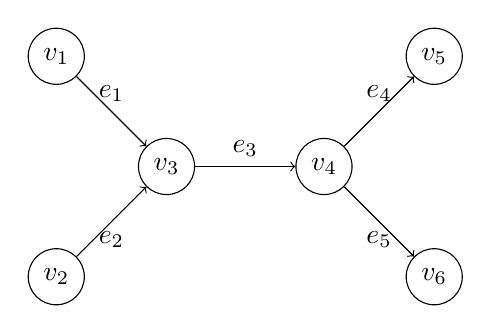
\begin{tikzpicture}
                % vertices
                \node[shape=circle,draw=black] (v1) at (-2.4,1.4) {$v_1$};
                \node[shape=circle,draw=black] (v5) at (2.4,1.4) {$v_5$};
                \node[shape=circle,draw=black] (v3) at (-1,0) {$v_3$};
                \node[shape=circle,draw=black] (v4) at (1,0) {$v_4$};
                \node[shape=circle,draw=black] (v2) at (-2.4,-1.4) {$v_2$};
                \node[shape=circle,draw=black] (v6) at (2.4,-1.4) {$v_6$};
                
                % edges
                \path [->](v1) edge node[above] {$e_1$} (v3);
                \path [->](v2) edge node[below] {$e_2$} (v3);
                \path [->](v3) edge node[above] {$e_3$} (v4);
                \path [->](v4) edge node[above] {$e_4$} (v5);
                \path [->](v4) edge node[below] {$e_5$} (v6);
            \end{tikzpicture}
            }
        \end{center}
    \end{figure}
    \begin{itemize}
        \item $T = 10$ and $\ell_e = 1$ for all $e \in \mathcal{E}$.
        \item $\varepsilon = 0.01$, $\partial_x V_e \left(t,x\right) = 1$ for all $\left(t,x\right) \in \left(0, 10\right) \times \left[0,1\right]$. 
        \item $\alpha_{v_1}\left(t\right) = 0.9$ and $\alpha_{v_2}\left(t\right) = 0.3$.
        \item $\beta_{v_5}\left(t\right) = 0.8$ and $\beta_{v_6}\left(t\right) = 0.1$. 
        \item $\rho_e\left(0,x\right) = 0$ for all $x \in \left[0, 1 \right]$ for each edge $e \in \mathcal{E}$.
        \item $\left\{ \left( t_e^i, x_e^i \right) \right\}_{i=1}^{4000}$, $\left\{ x_{e,0}^i \right\}_{i=1}^{1000}$, $\left\{ t_{0,b}^i \right\}_{i=1}^{1000}$ for $v=1$ and $\left\{ t_{0,b}^i \right\}_{i=1}^{1000}$ for $v=0$ randomly chosen (normal distribution).  
    \end{itemize}
\end{frame}


\begin{frame}{Results}
    Implemented with \lstinline!Python 3.8.8! \\
    \vspace{5mm}
    $\operatorname{fnn}_{\theta_e} \colon \; L = 3; \; n_0 = 2; \; n_1, n_2 = 10; \; n_3 = 1; \; \sigma_l\left( \cdot \right) = \tanh \left( \cdot \right)$. \\ 
    $\operatorname{R}_{\theta_e} \colon \; L = 3; \; n_0 = 2; \; m = 12; \; h = 1; \; \sigma_l\left( \cdot \right) = \tanh \left( \cdot \right)$. \\ 
    $\operatorname{FNN}_{\theta} \colon \; L = 4; \; n_0 = 2; \; n_1, n_2, n_3 = 20; \; n_4 = 5; \; \sigma_l\left( \cdot \right) = \tanh \left( \cdot \right)$. \\ 
    \vspace{5mm}
    Results after $2 \cdot 10^{3}$ iterations with ADAM optimizer and $5 \cdot 10^{4}$ iterations with L-BFGS-B optimizer. 
    \begin{figure}[H]
        \begin{center}
            \resizebox{!}{!}
            {
                \begin{tabular}{l l l l }
                    \toprule
                    Neural Network & $\operatorname{fnn}_{\theta_e}$ & $\operatorname{R}_{\theta_e}$ & $\operatorname{FNN}_{\theta}$  \\ 
                    \midrule
                    $\Phi_{\theta} \left( \operatorname{X} \right)$ & $3.63 \cdot 10^{-4}$ & $3.05 \cdot 10^{-2}$ & $4.46 \cdot 10^{-4}$  \\
                    \midrule
                    $L^2$-Error* & $275.64$ & $1530.23$ & $430.45$ \\ 
                    \midrule
                    Computational Time & $\sim 62 \ min$ & $\sim 70 \ min$ & $\sim 87 \ min$ \\ 
                    \bottomrule
                \end{tabular}
            }
        \end{center}
    \end{figure}
    *with respect to values generated with $FVM$ at the same grid points ($25 \cdot 10^{6}$).
\end{frame}



\begin{frame}{Results}
    \begin{figure}[H]
        \begin{center}
            \begin{subfigure}[b]{0.4\textwidth}
                \begin{center}
                    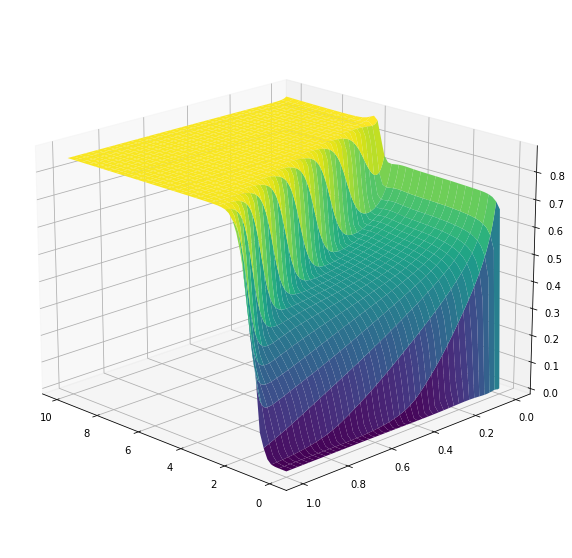
\includegraphics[scale=0.25]{img/Kante1.png}
                \end{center}
                \caption{$\operatorname{fnn}_{\theta_{e_1}}$}
            \end{subfigure} \hspace{10mm}
            \begin{subfigure}[b]{0.4\textwidth}
                \begin{center}
                    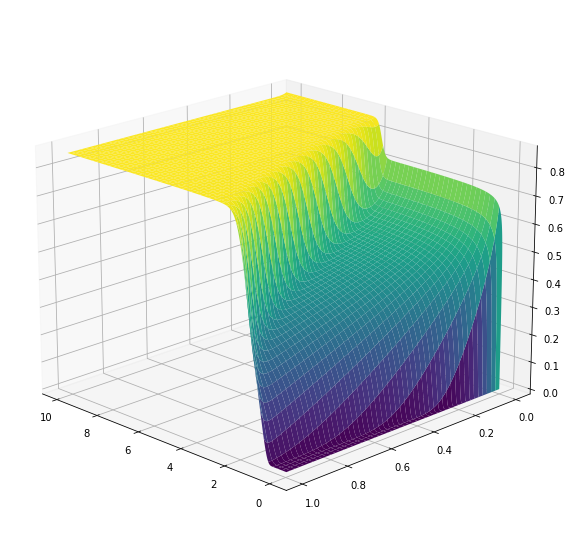
\includegraphics[scale=0.25]{img/FVM1.png}
                \end{center}
                \caption{$FVM$ on $e_1$}
            \end{subfigure}
        \end{center}
    \end{figure}
\end{frame}



\begin{frame}{Results}
    \begin{figure}[H]
        \begin{center}
            \begin{subfigure}[b]{0.4\textwidth}
                \begin{center}
                    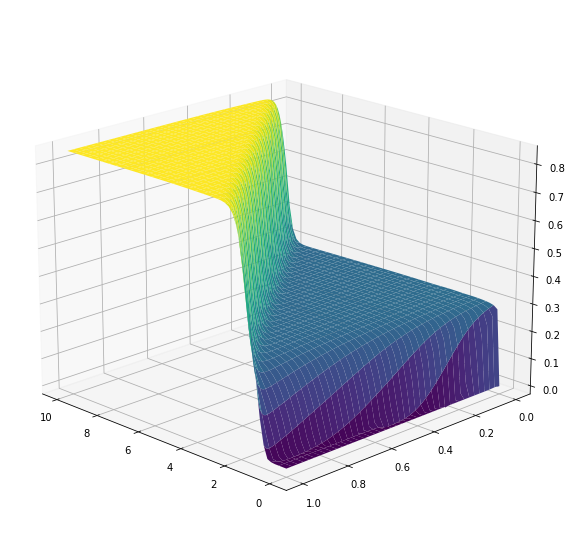
\includegraphics[scale=0.25]{img/Kante2.png}
                \end{center}
                \caption{$\operatorname{fnn}_{\theta_{e_2}}$}
            \end{subfigure} \hspace{10mm}
            \begin{subfigure}[b]{0.4\textwidth}
                \begin{center}
                    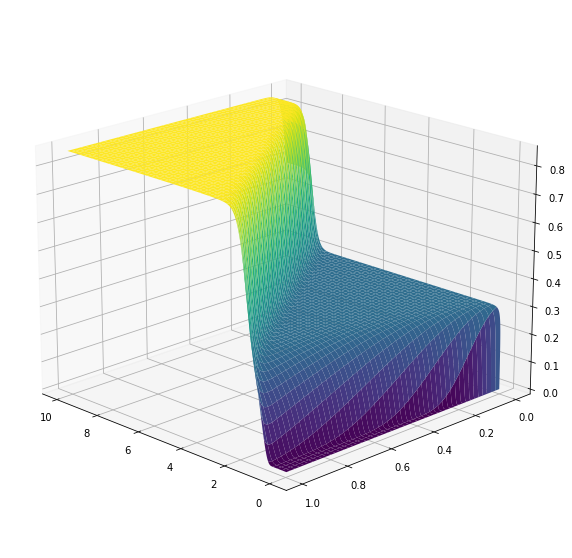
\includegraphics[scale=0.25]{img/FVM2.png}
                \end{center}
                \caption{$FVM$ on $e_2$}
            \end{subfigure}
        \end{center}
    \end{figure}
\end{frame}



\begin{frame}{Results}
    \begin{figure}[H]
        \begin{center}
            \begin{subfigure}[b]{0.4\textwidth}
                \begin{center}
                    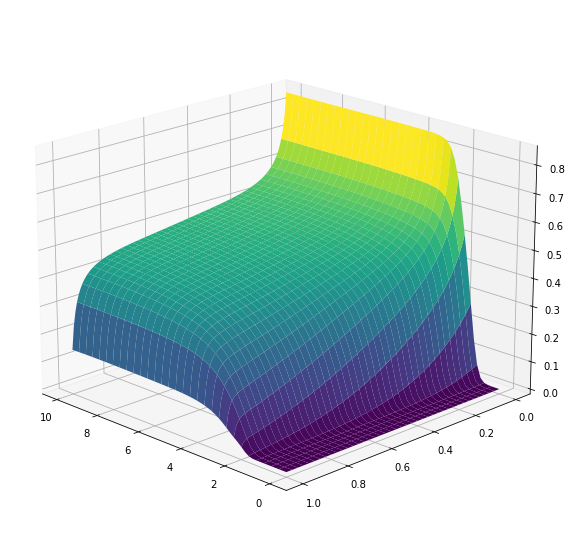
\includegraphics[scale=0.25]{img/Kante3.png}
                \end{center}
                \caption{$\operatorname{fnn}_{\theta_{e_3}}$}
            \end{subfigure} \hspace{10mm}
            \begin{subfigure}[b]{0.4\textwidth}
                \begin{center}
                    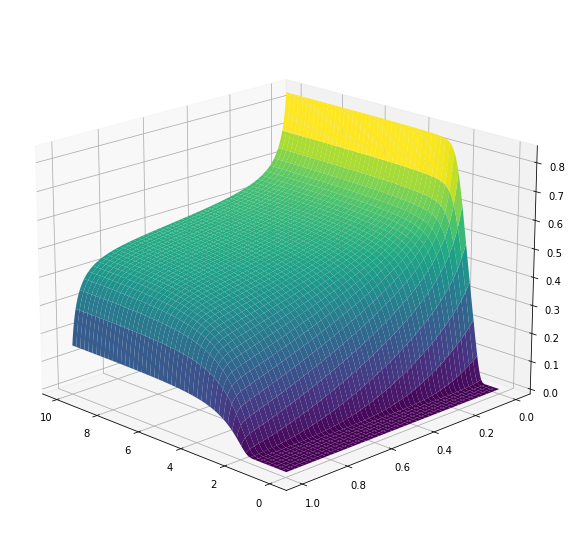
\includegraphics[scale=0.25]{img/FVM3.png}
                \end{center}
                \caption{$FVM$ on $e_3$}
            \end{subfigure}
        \end{center}
    \end{figure}
\end{frame}



\begin{frame}{Results}
    \begin{figure}[H]
        \begin{center}
            \begin{subfigure}[b]{0.4\textwidth}
                \begin{center}
                    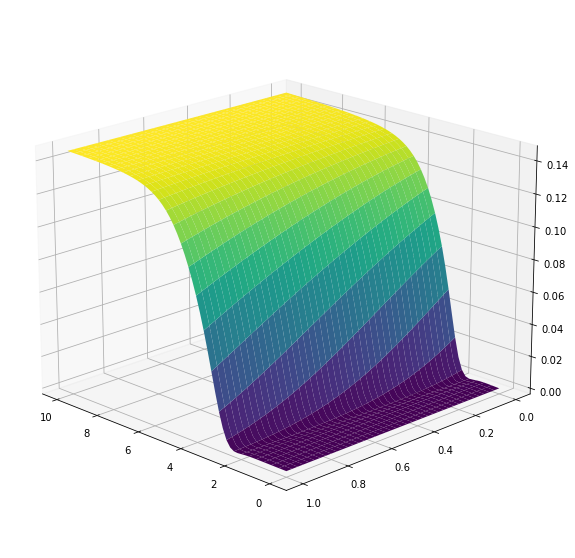
\includegraphics[scale=0.25]{img/Kante4.png}
                \end{center}
                \caption{$\operatorname{fnn}_{\theta_{e_4}}$}
            \end{subfigure} \hspace{10mm}
            \begin{subfigure}[b]{0.4\textwidth}
                \begin{center}
                    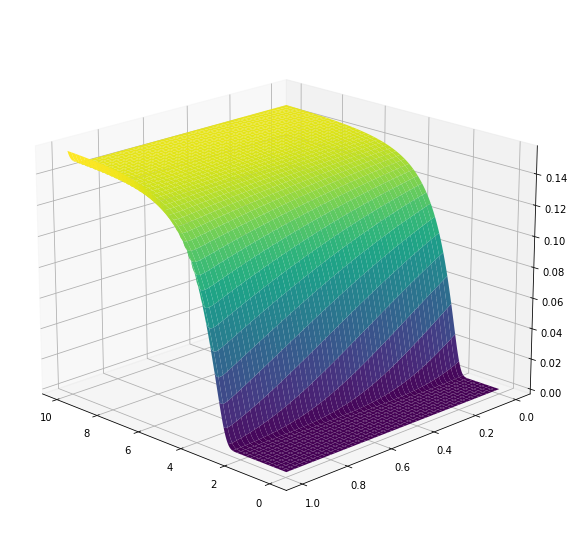
\includegraphics[scale=0.25]{img/FVM4.png}
                \end{center}
                \caption{$FVM$ on $e_4$}
            \end{subfigure}
        \end{center}
    \end{figure}
\end{frame}



\begin{frame}{Results}
    \begin{figure}[H]
        \begin{center}
            \begin{subfigure}[b]{0.4\textwidth}
                \begin{center}
                    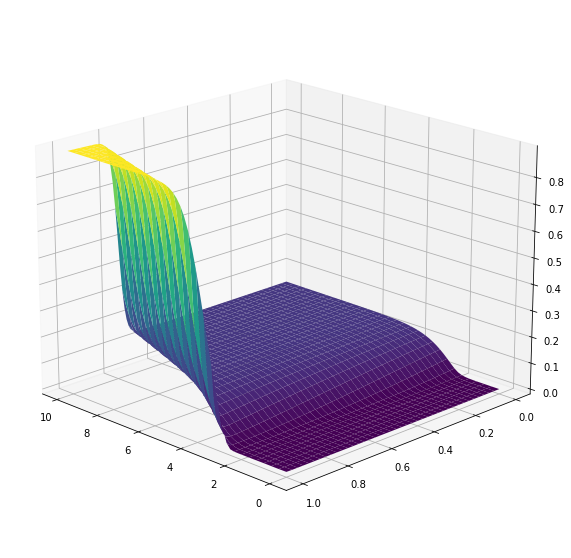
\includegraphics[scale=0.25]{img/Kante5.png}
                \end{center}
                \caption{$\operatorname{fnn}_{\theta_{e_5}}$}
            \end{subfigure} \hspace{10mm}
            \begin{subfigure}[b]{0.4\textwidth}
                \begin{center}
                    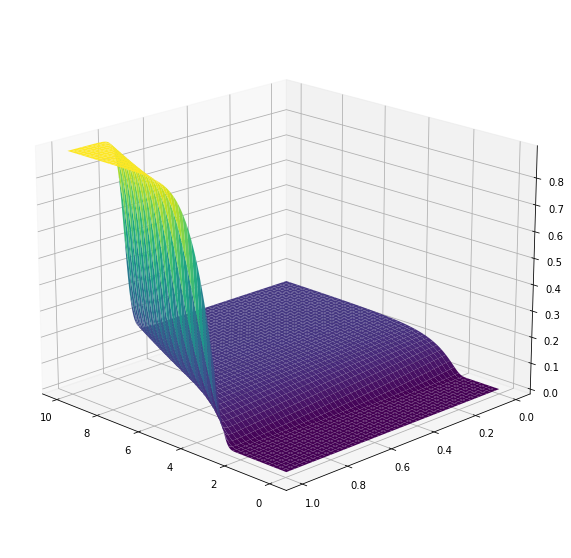
\includegraphics[scale=0.25]{img/FVM5.png}
                \end{center}
                \caption{$FVM$ on $e_5$}
            \end{subfigure}
        \end{center}
    \end{figure}
\end{frame}


\section{Explicit Derivatives vs. \\ Automatic Differentiation}



\begin{frame}{The desire to make the code work faster}
    \vspace{-1\baselineskip}\hfill{\tiny{[Ruthotto et al., 2020]}} \\
    \textbf{Idea}: Instead of automatic differentiation, use explicitly calculated derivatives in the misfit terms. This could reduce the computational time. \\
    \vspace{3mm}
    We have implemented vectorised recursive iterations for the calculation of$\ldots$ \\
    \begin{itemize}
        \item $\nabla \operatorname{fnn}_{\theta_e} \left( x^0 \right) \in \mathbb{R}^{n_0}$ and $\nabla^2 \operatorname{fnn}_{\theta_e} \left( x^0 \right) \in \mathbb{R}^{n_0 \times n_0}$,
        \item $\nabla \operatorname{R}_{\theta_e} \left( x^0 \right) \in \mathbb{R}^{n_0}$ and $\nabla^2 \operatorname{R}_{\theta_e} \left( x^0 \right) \in \mathbb{R}^{n_0 \times n_0}$,
        \item $\mathrm{J} \left[ \operatorname{FNN}_{\theta} \right]\left(x^0\right) \in \mathbb{R}^{n_L \times n_0}$ and $\mathrm{H} \left[\operatorname{FNN}_{\theta} \right]\left(x^0\right) \in \mathbb{R}^{n_L \times n_0 \times n_0}$.
    \end{itemize}
    \vspace{3mm}
    \textbf{Competitor}: \lstinline!tf.GradientTape! from \lstinline!TensorFlow!. \\
    \vspace{7mm}
    Results from numerical experiments: \textbf{it got even worse}. 
\end{frame}



\section{Conclusion \& Outlook}



\begin{frame}{Conclusion}
    \begin{itemize}
        \item It is possible to approximate the solution of the set of drift-diffusion equations using PINNs.
        \item It is very slow.
        \item Explicit derivatives have not been useful (so far).
        \item New research questions arose!
    \end{itemize}
\end{frame}

\begin{frame}{Outlook}
    \textbf{We're not done yet!}
    \begin{itemize}
        \item Hyperparameter optimization (has failed so far). 
        \item Another cost function?
        \item Another approach?
    \end{itemize}
\end{frame}

\begin{frame}
    \begin{center}
        \Huge{Thank you for your attention!} \\
        \huge{Questions?}
    \end{center}
\end{frame}



\begin{frame}{Sketch}
    
\end{frame}

\begin{frame}{Sketch}
    
\end{frame}

\begin{frame}{Sketch}
    
\end{frame}



\begin{frame}{Another cost function 1}
    \begin{equation*}
        \begin{aligned} 
            \Phi_{\theta} \left( \operatorname{X} \right)  = & \quad \frac{1}{\abs{\mathcal{E}}} \sum_{e \in \mathcal{E}}  \left(  \phi_{e,r}  \left( X_{e,r} \right) + \phi_{e,0}  \left( X_{e,0} \right)  \right) + \\
            & + \frac{1}{\abs{\mathcal{V}_\mathcal{K}}} \sum_{v \in \mathcal{V}_\mathcal{K}}  \left(  \phi_{v,K}  \left( X_{v,b} \right) + \phi_{v,c} \left( X_{v,b} \right)  \right) + \\
            & + \frac{1}{\abs{\mathcal{V}_\mathcal{D}}} \sum_{v \in \mathcal{V}_\mathcal{D}} \phi_{v,D} \left( X_{v,b} \right).
        \end{aligned}
    \end{equation*}
\end{frame}



\begin{frame}{Another cost function 2}
    Replace for each $v \in \mathcal{V}_{\mathcal{K}}$ the continuity misfit term
    \begin{equation*} 
        \phi_{v,c}  \left( X_{v,b} \right) \coloneqq \frac{1}{n_b} \sum_{e \in \mathcal{E}_v} \sum_{i=1}^{n_b} \left(  \rho_{\theta_e}  \left( t_{v,b}^i, v \right) - \rho_{v}^i \right)^2
    \end{equation*}
    with
    \begin{equation*} 
        \phi_{v,c}  \left( X_{v,b} \right) \coloneqq \frac{1}{n_b}  \sum_{i=1}^{n_b} \left( \sum_{e \in \mathcal{E}_v} \left( \rho_{\theta_e}  \left( t_{v,b}^i, v \right) - \frac{1}{\abs{\mathcal{E}_v}} \sum_{e \in \mathcal{E}_v} \rho_{\theta_e}  \left( t_{v,b}^i, v \right) \right) \right)^2.
    \end{equation*}
\end{frame}



\begin{frame}{Another approach: cost function for each egde}
    We minimize in the learning phase for each edge $e \in \mathcal{E}$ the following cost function with respect to $\theta_e$
    \begin{equation*}
        \phi_{\theta_e} \left( \operatorname{X} \right) \coloneqq \phi_{e,r}  \left( X_e \right) + \phi_{e,0}  \left( X_{e,0} \right) + \phi_{v^{\operatorname{o}}_e}(X_{v,b}) + \phi_{v^{\operatorname{t}}_e}(X_{v,b})
    \end{equation*}
    with 
    \begin{equation*}
        \phi_{v}(X_{v,b}) = \begin{cases} \phi_{v,K}  \left( X_{v,b} \right) +  \phi_{v,c}  \left( X_{v,b} \right)& \text{if } v \in \mathcal{V}_{\mathcal{K}}, \\ \phi_{v,D}  \left( X_{v,b} \right) & \text{if } v \in \mathcal{V}_{\mathcal{D}}. \end{cases}
    \end{equation*}
\end{frame}


\begin{frame}{Another approach: cost function for each vertex}
    We minimize in the learning phase for each vertex $v \in \mathcal{V}$ the following cost function with respect to $\theta_v$
    \begin{equation*}
        \phi_{\theta_v} \left( \operatorname{X} \right) \coloneqq \phi_{v}(X_{v,b}) + \sum_{e \in \mathcal{E}_v} \left( \phi_{e,r}  \left( X_e \right) + \phi_{e,0}  \left( X_{e,0} \right) \right)
    \end{equation*}
    with 
    \begin{equation*}
        \phi_{v}(X_{v,b}) = \begin{cases} \phi_{v,K}  \left( X_{v,b} \right) +  \phi_{v,c}  \left( X_{v,b} \right)& \text{if } v \in \mathcal{V}_{\mathcal{K}}, \\ \phi_{v,D}  \left( X_{v,b} \right) & \text{if } v \in \mathcal{V}_{\mathcal{D}}. \end{cases}
    \end{equation*}
    \vspace{5mm}

    Using $f_{\theta_v} \colon \mathbb{R}^2 \to \mathbb{R}^{\abs{\mathcal{E}_v}}$.
\end{frame}



\begin{frame}{Explicit derivatives FNN (one-dimensional)}

    $\operatorname{fnn}_{\theta_e} \colon \; L = 4; \; n_0 = 2; \; n_1, n_2, n_3 = 10; \; n_4 = 1; \; \sigma_l\left( \cdot \right) = \operatorname{sigmoid} \left( \cdot \right)$. \\ 
    \vspace{5mm}
    \begin{table}[H]
        \resizebox{!}{!}
        {
            \begin{tabular}{l l l l l }
                \toprule
                Derivative & \multicolumn{2}{c}{$\nabla f_{\theta} \left( x^0 \right)$}& \multicolumn{2}{c}{$\nabla^2 f_{\theta} \left(x^0\right)$} \\ 
                \midrule
                Method & Explicit & $AD$ & Explicit & $AD$ \\ 
                \midrule
                $N = 100$ & $6.88$ & $1.22$ & $76.95$ & $9.68$ \\ 
                \midrule
                $N = 1000$ & $8.75$ & $1.31$ & $773.53$ & $14.06$ \\ 
                \midrule
                $N = 10000$ & $16.33$ & $3.46$ & $8379.95$ & $28.10$ \\ 
                \bottomrule
            \end{tabular}
        }
    \end{table}
\end{frame}


\begin{frame}{Explicit derivatives ResNet}

    $\operatorname{R}_{\theta_e} \colon \; L = 4; \; n_0 = 2; \; m = 10; \; h = 1; \; \sigma_l\left( \cdot \right) = \operatorname{sigmoid} \left( \cdot \right)$. \\  
    \vspace{5mm}
    \begin{table}[H]
        \resizebox{!}{!}
        {
            \begin{tabular}{l l l l l }
                \toprule
                Derivative & \multicolumn{2}{c}{$\nabla R_{\theta} \left(x^0 \right)$}& \multicolumn{2}{c}{$\nabla^2 R_{\theta} \left(x^0 \right)$} \\ 
                \midrule
                Method & Explicit & $AD$ & Explicit & $AD$ \\ 
                \midrule
                $N = 100$ & $13.66$ & $5.12$ & $255.88$ & $27.74$ \\ 
                \midrule
                $N = 1000$ & $15.95$ & $6.49$ & $2371.42$ & $28.11$ \\ 
                \midrule
                $N = 10000$ & $21.80$ & $12.18$ & $26053.93$ & $70.63$ \\ 
                \bottomrule
            \end{tabular}
        }
    \end{table}
\end{frame}



\begin{frame}{Explicit derivatives FNN (multi-dimensional)}

    $\operatorname{FNN}_{\theta} \colon \; L = 4; \; n_0 = 2; \; n_1, n_2, n_3 = 10; \; n_4 = 1; \; \sigma_l\left( \cdot \right) = \operatorname{sigmoid} \left( \cdot \right)$. \\ 
    \vspace{5mm}
    \begin{table}[H]
        \resizebox{!}{!}
        {
            \begin{tabular}{l l l l l }
                \toprule
                Derivative & \multicolumn{2}{c}{$\mathrm{J} \left[ F_{\theta} \right]\left(x^0\right)$}& \multicolumn{2}{c}{$\mathrm{H} \left[F_{\theta} \right]\left(x^0\right)$} \\ 
                \midrule
                Method & Explicit & $AD$ & Explicit & $AD$ \\ 
                \midrule
                $N = 100$ & $15.10$ & $13.30$ & $323.99$ & $57.72$ \\ 
                \midrule
                $N = 1000$ & $18.42$ & $16.86$ & $3292.42$ & $88.82$ \\ 
                \midrule
                $N = 10000$ & $46.59$ & $52.27$ & $37580.87$ & $340.43$ \\ 
                \bottomrule
            \end{tabular}
        }
    \end{table}
\end{frame}




\begin{frame}
    \begin{equation*} 
        \begin{aligned}
            \nabla f_{\theta, i} \left(x^0\right) & = \delta^1 \\
            \delta^1 & = {W^{1}}^{\mathrm{T}} \cdot D^{1} \cdot \delta^2 \in \mathbb{R}^{n_0}, \\
            \vdots & \\
            \delta^l & = {W^{l}}^{\mathrm{T}} \cdot D^{l} \cdot \delta^{l+1} \in \mathbb{R}^{n_{l-1}}, \\
            \vdots & \\
            \delta^{L} & = {W^L}^{\mathrm{T}} \cdot D^{L} \in \mathbb{R}^{n_{L-1}}.
        \end{aligned} 
    \end{equation*} 
\end{frame}



\begin{frame}
    \begin{equation*}
        \begin{aligned}
            \nabla^{2} f_{\theta, i} \left(x^0\right) & = \eta^{1} \in \mathbb{R}^{n_0 \times n_0} \\
            \eta^{1} & = {W^{1}}^{\mathrm{T}} \left( H^{1} + D^{1} \eta^{2} D^{1} \right) W^{1} \\
            & \vdots \\
            \eta^{l} & = {W^{l}}^{\mathrm{T}} \left( H^{l} + D^{l} \eta^{l+1} D^{l} \right) W^{l} \in \mathbb{R}^{n_{l-1} \times n_{l-1}} \\
            & \vdots \\
            \eta^{L} & = {W^L}^{\mathrm{T}} H^{L} W^L \in \mathbb{R}^{n_{L-1} \times n_{L-1}}.
        \end{aligned}
    \end{equation*}
\end{frame}



\begin{frame}
    \begin{equation*}
        \begin{aligned}
            \nabla \left( {x^{L}}^{\mathrm{T}} w \right) & = \delta^{1} \in \mathbb{R}^{n_0}  \\
            \delta^{1} & = {W^{1}}^{\mathrm{T}} D^{1} \, \delta^{2} \in \mathbb{R}^{n_0} \\
            \delta^{2} & = \delta^{3} + h \, {W^{2}}^{\mathrm{T}} D^{2} \, \delta^{3} \in \mathbb{R}^{m} \\
            &\vdots\\
            \delta^{l} & = \delta^{l+1} + h \, {W^{l}}^{\mathrm{T}} D^{l} \, \delta^{l+1} \in \mathbb{R}^{m} \\
            &\vdots\\
            \delta^{L-1} & = \delta^{L} + h \, {W^{L-1}}^{\mathrm{T}} D^{L-1} \, \delta^{L} \in \mathbb{R}^{m} \\
            \delta^{L} & = w + h \, {W^{L}}^{\mathrm{T}} D^{L} \, w \in \mathbb{R}^{m}.
        \end{aligned}   
    \end{equation*}
\end{frame}



\begin{frame}
    \begin{equation*}
        \begin{aligned}
            \nabla^2 \left( {x^{L}}^{\mathrm{T}} w \right) & = \eta^{1} \in \mathbb{R}^{n_0 \times n_0}  \\
            \eta^{1} & = {W^{1}}^{\mathrm{T}} \left( H^{1} + D^{1} \eta^{2} D^{1} \right) W^{1} \in \mathbb{R}^{n_0 \times n_0} \\
            \eta^{2} & = h \, {W^{2}}^{\mathrm{T}} H^2 W^{l} + \left( I + h \, {W^{2}}^{\mathrm{T}} D^{2} \right) \, \eta^{3} \, \left( I + h \,  D^{2} W^{2} \right) \in \mathbb{R}^{m \times m}\\ 
            &\vdots\\
            \eta^{l} & = h \, {W^{l}}^{\mathrm{T}} H^{l} W^{l} + \left( I + h \, {W^{l}}^{\mathrm{T}} D^{l} \right) \, \eta^{l+1} \, \left( I + h \,  D^{l} {W^{l}} \right) \in \mathbb{R}^{m \times m} \\ 
            &\vdots\\
            \eta^{L-1} & = h \, {W^{L-1}}^{\mathrm{T}} H^{L-1} W^{L-1} + \left( I + h \, {W^{L-1}}^{\mathrm{T}} D^{L-1} \right) \, \eta^{L-2} \, \left( I + h \,  D^{L-1} W^{L-1} \right) \in \mathbb{R}^{m \times m} \\ 
            \eta^{L} &  = {W^{L}}^{\mathrm{T}} H^{L} W^{L}.
        \end{aligned}
    \end{equation*}
\end{frame}



\begin{frame}
    \begin{figure}[H]
        \begin{center}
            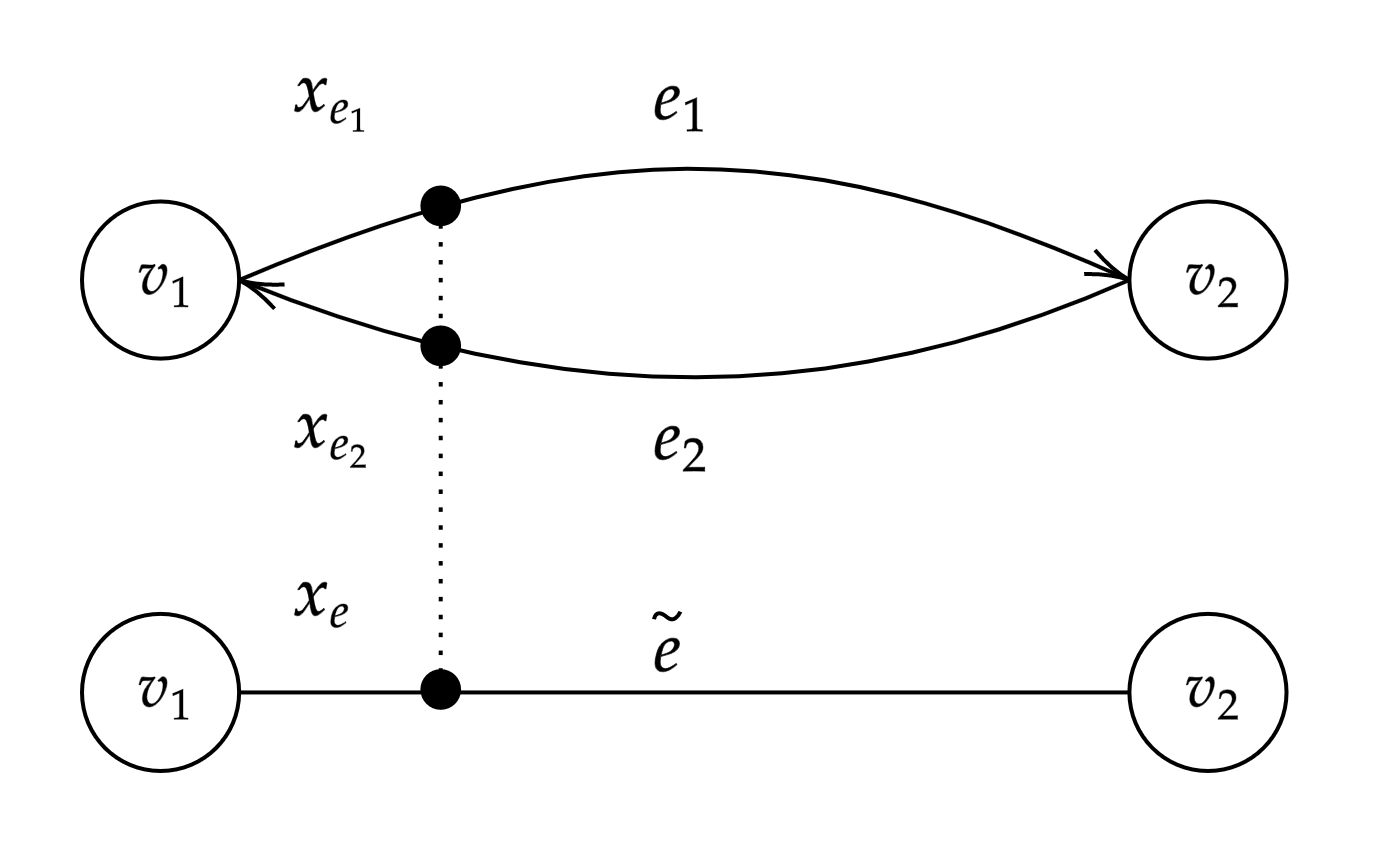
\includegraphics[scale=0.25]{img/diagram-20220315 (2).png}
        \end{center}
    \end{figure}
\end{frame}




\begin{comment}
    
\begin{frame}
    \begin{itemize}
        \item Adjacency: $v_1, v_2 \in \mathcal{V}$ \\ $v_1 \sim v_2 \Leftrightarrow \exists e \in \mathcal{E}$ s.t. $v_2$ can be reached from $v_1$ via this edge $e$. \\
        \begin{equation*}
          A^{\Gamma} = 
          \begin{blockarray}{ccccc}
              v_1 & v_2 & v_3 & v_4 \\
              \begin{block}{(cccc)c}
                  0 & 1 & 0 & 0 & v_1 \\
                  0 & 0 & 0 & 1 & v_2 \\
                  0 & 1 & 0 & 1 & v_3 \\
                  0 & 1 & 0 & 0 & v_4 \\
              \end{block}
          \end{blockarray}
      \end{equation*}
    \end{itemize}
    \textbf{Metric Graph}:
        \begin{itemize}
            \item $\forall e \in \mathcal{E} \colon \, \exists \ell_e > 0$.
            \item $\ell_{e_1} = \ell_{\overline{e_1}} = \ell_{e_2} = \ell_{\tilde{e}}$.
            \item $x_{e_1} \in [0, \ell_{e_1}] \colon \, x_{e_1} = \ell_{e_2} - x_{e_2}$.
            \item $\operatorname{dist}(v_i, v_j) = \sum^{N}_{k = 1} \ell_{e_k}$, \\ where $\left\{ e_k \right\}_{k = 1, \ldots, N}$ is path of minimal length.
        \end{itemize}
\end{frame}

\end{comment}

\end{document}
